\documentclass{extarticle}
\usepackage{listings}
\usepackage{graphicx}
\usepackage{float}
% \usepackage{courier}

\usepackage{fontspec}
\setsansfont{Ubuntu}% Ubuntu as sans - use \sffamily or \textsf{} as normal
\setmonofont{JetBrainsMono Nerd Font Mono}% Ubuntu Mono as 'typewriter' - use \ttfamily or \texttt{}

\usepackage[a4paper,
            bindingoffset=0.2in,
            left=1cm,
            right=1cm,
            top=1in,
            bottom=1in,
            footskip=.25in]{geometry}

\usepackage{hyperref}
\hypersetup{
    colorlinks, citecolor=black, filecolor=black,
    linkcolor=black, urlcolor=black
}

\usepackage{xcolor}
\definecolor{mygreen}{rgb}{0.05,0.15,0.11}
\definecolor{mygray}{rgb}{0.9,0.9,0.9}
\definecolor{mymauve}{rgb}{0.58,0,0.82}

\lstset{
%   backgroundcolor=\color{mygray}, 
  basicstyle=\ttfamily,
  breakatwhitespace=false,
  breaklines=true,
%   commentstyle=\itshape,
  keepspaces=true,
  keywordstyle=\bfseries,
  morekeywords={*,...},
  showspaces=false,
  showstringspaces=false,
  showtabs=false,
%   stringstyle=\color{blue},
  tabsize=2,
%   numbers=left,
  rulecolor=\color{black},
  postbreak=\mbox{\textcolor{red}{$\hookrightarrow$}\space}
}

\title{Web Development Assignment 1}
\author{Shivanshu}

\begin{document}
\pagenumbering{gobble}

\centerline{\bfseries \Huge Assignment 1}
\section*{Question 1}

Write the HTML code for the following Table and write some text in each cell.

\begin{figure}[H]
    \caption{Table 1}
    \centering
    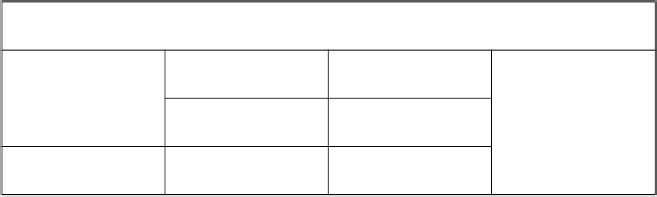
\includegraphics[width=15cm]{./img/a.jpg}
\end{figure}

\begin{figure}[H]
    \caption{Table 1}
    \centering
    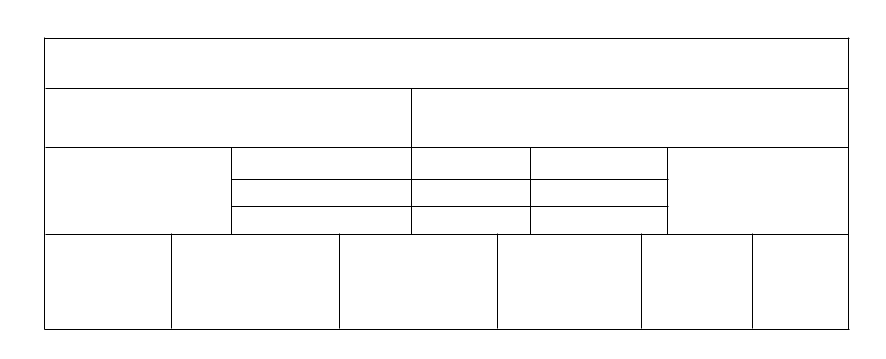
\includegraphics[width=15cm]{./img/aa.png}
\end{figure}

\newpage
\subsection*{Code}
\lstinputlisting[language=html]{1/1.html}

\newpage
\subsection*{Code}
\lstinputlisting[language=html]{2/2.html}

\newpage
\subsection*{Output}
\begin{figure}[H]
    \caption{Table Preview}
    \centering
    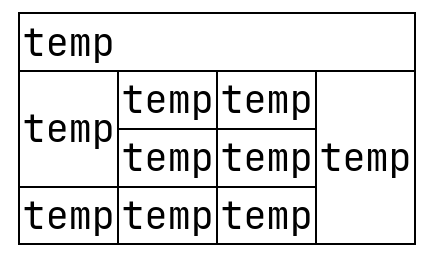
\includegraphics[width=5cm]{1/1.png}
\end{figure}

\begin{figure}[H]
    \caption{Table Preview}
    \centering
    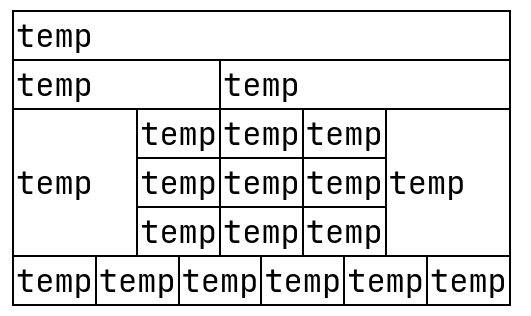
\includegraphics[width=5cm]{2/2.png}
\end{figure}

\newpage
\section*{Question 2}

Write the HTML code for the following Table.

\begin{figure}[H]
    \caption{Table 3}
    \centering
    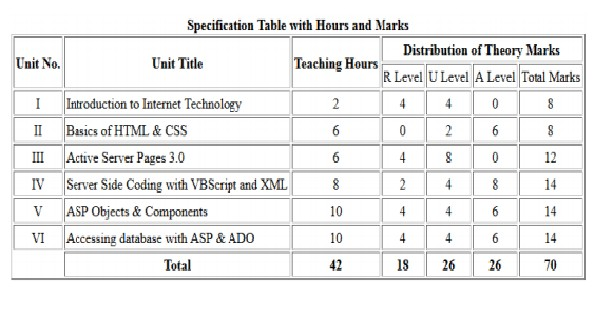
\includegraphics[width=15cm]{./img/b.jpg}
\end{figure}

\newpage
\subsection*{Code}
\lstinputlisting[language=html]{3/3.html}

\newpage
\subsection*{Output}
\begin{figure}[H]
    \caption{Table Preview}
    \centering
    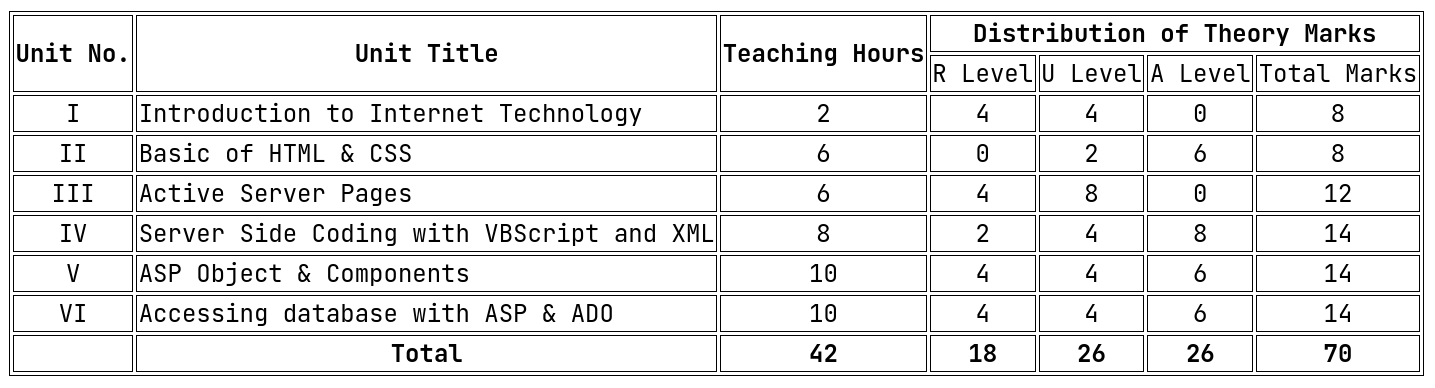
\includegraphics[width=16cm]{3/3.png}
\end{figure}

\newpage
\section*{Question 3}

Write the HTML code, which defines all the formatting

\begin{figure}[H]
    \caption{Table 3}
    \centering
    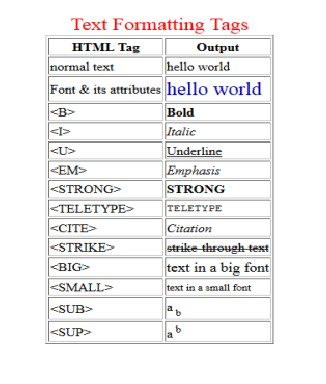
\includegraphics[width=13cm]{./img/c.jpg}
\end{figure}

\newpage
\subsection*{Code}
\lstinputlisting[language=html]{4/4.html}

\newpage
\subsection*{Output}
\begin{figure}[H]
    \caption{Table Preview}
    \centering
    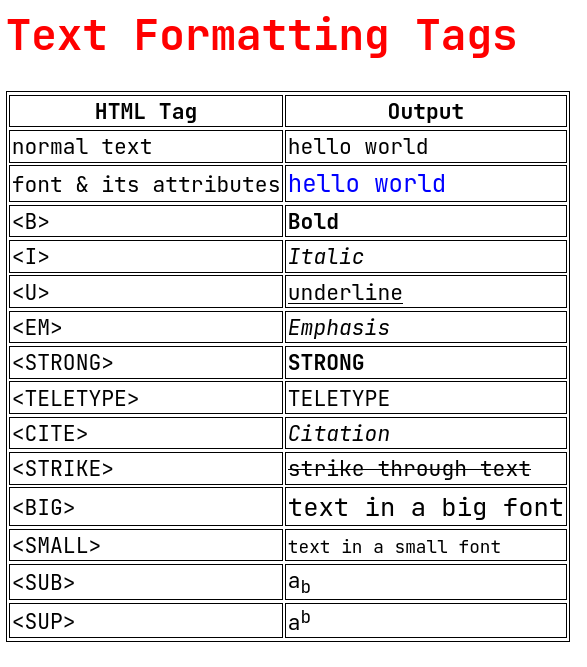
\includegraphics[width=10cm]{4/4.png}
\end{figure}

\newpage
\section*{Question 4}

\subsection*{Code}

Write the HTML code to display Uttarakhand map.
And also display districts detail after clicking on a
particular district.

\begin{figure}[H]
    \caption{Map}
    \centering
    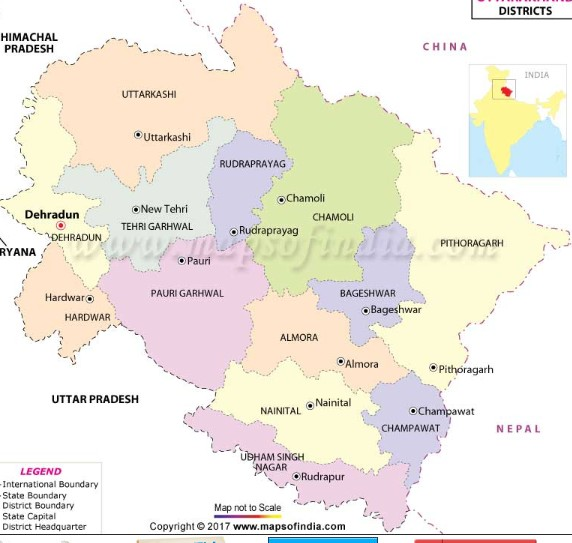
\includegraphics[width=10cm]{./img/d.jpg}
\end{figure}

\newpage
\lstinputlisting[language=html]{5/5.html}

\newpage
\subsection*{Output}
\begin{figure}[H]
    \caption{Map}
    \centering
    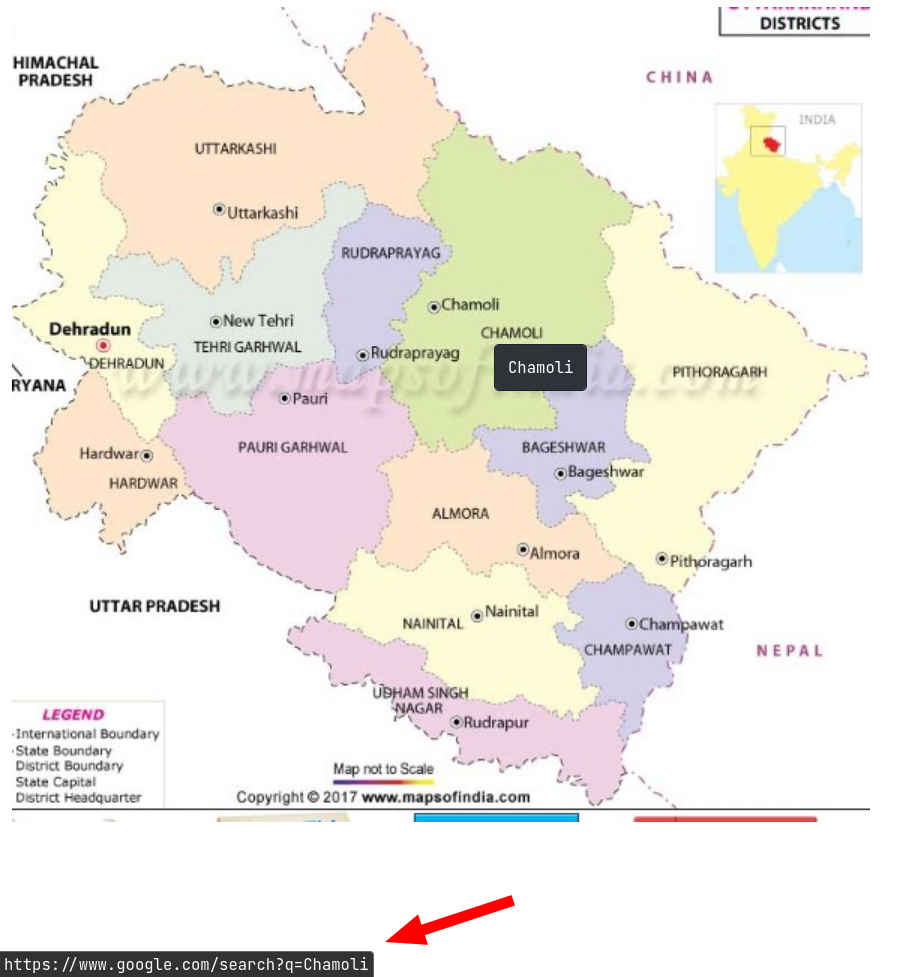
\includegraphics[width=10cm]{5/5.png}
\end{figure}

\end{document}